%
% Complete documentation on the extended LaTeX markup used for Insight
% documentation is available in ``Documenting Insight'', which is part
% of the standard documentation for Insight.  It may be found online
% at:
%
%     http://www.itk.org/

\documentclass{InsightArticle}


%%%%%%%%%%%%%%%%%%%%%%%%%%%%%%%%%%%%%%%%%%%%%%%%%%%%%%%%%%%%%%%%%%
%
%  hyperref should be the last package to be loaded.
%
%%%%%%%%%%%%%%%%%%%%%%%%%%%%%%%%%%%%%%%%%%%%%%%%%%%%%%%%%%%%%%%%%%
\usepackage[dvips,
bookmarks,
bookmarksopen,
backref,
colorlinks,linkcolor={blue},citecolor={blue},urlcolor={blue},
]{hyperref}
% to be able to use options in graphics
\usepackage{graphicx}
% for pseudo code
\usepackage{listings}
% subfigures
\usepackage{subfigure}
\usepackage{pseudocode}


%  This is a template for Papers to the Insight Journal. 
%  It is comparable to a technical report format.

% The title should be descriptive enough for people to be able to find
% the relevant document. 
\title{FFT based convolution}

% Increment the release number whenever significant changes are made.
% The author and/or editor can define 'significant' however they like.
% \release{0.00}

% At minimum, give your name and an email address.  You can include a
% snail-mail address if you like.
\author{Ga\"etan Lehmann{$^1$}}
\authoraddress{{$^1$}INRA, UMR 1198; ENVA; CNRS, FRE 2857, Biologie du
D\'eveloppement et 
Reproduction, Jouy en Josas, F-78350, France.}

\begin{document}
\maketitle

\ifhtml
\chapter*{Front Matter\label{front}}
\fi


\begin{abstract}
\noindent

The Fourier transform of the convolution of two images is equal to the product of their
Fourier transform. With this definition, it is possible to create a convolution filter
based on the Fast Fourier Transform (FFT). The interesting complexity characteristics of
this transform gives a very efficient convolution filter for large kernel images.

This paper provides such a filter, as well as a detailed description of the implementation
choices and a comparison with the "simple" itk::ConvolutionImageFilter.

\end{abstract}

\tableofcontents

\section{Introduction}

The convolution of two image is a very cpu demanding task, with a complexity of $O(N \times M)$ where $N$ is
the number of pixel of the first image and $M$ the number of pixels of the second. Usually, the size
of one of the image is a lot smaller than the one of the other -- the smaller is often called the
kernel. The quite small size of the kernel makes the convolution computable in a very usable time,
but when the size of the kernel grows, the computation time quickly becomes impraticable.

Fortunately, the convolution of two images is simply the product of those two images pixel wise in
the frequency domain, with a complexity of $O(max(N, M))$. The size of the kernel, which is usually
way smaller than the image, has no effect on the computation time, so the complexity is simply $O(N)$.
The cost of the Fourier Transform
can be quite high however -- that's why the FFT based convolution is more efficient only for big
kernel images.

\section{FFT based convolution step by step}

The FFT based convolution requires several step to be performed. They are detailed one by one.

\subsection{Padding}

The image to convolve and the kernel will be padded with for several reasons:
\begin{itemize}
  \item to make their size match. This is required to perform the multiplication in the frequency
  domain.
  \item  to avoid the border effects. Because the FFT considere the image as a cyclic signal, the
  image must be padded to avoid the border effects. The final image size for all the dimensions
  must be at least $P+Q-1$, where $P$ is the size of the first image on a dimension and $Q$ the size
  of the other image on the same dimension.
  \item to make the FFT possible, or to enhance its performance. Some FFT implementations, like the
  VNL one, can only be run on an image where the size on all the dimensions are a power of two.
  Some other implementations, like FFTW's one, are performing very differently depending on the
  size of the image. Adding a few more pixels on the border of the image can lead them to perform
  a lot better, as shown in chapter \ref{perf:gpf}.
\end{itemize}

The kernel is always padded with zeros, but the image to convolve can be padded in several ways:
\begin{itemize}
 \item zeros -- while simple, this method may show darkened border in the convolved image;
 \item zero flux Neumann -- this method extends the pixels on the image border in the padded zone, and
       is quite efficient in keeping the border effect low;
 \item mirror -- the image is padded with a mirror of the image. This is also a quite good way to
       keep the border effect low;
 \item wrap -- the opposite border of the image is copied in the padded zone. This may be useful to
       keep the circular behavior of the FFT, while still padding to fit the size requirement of the
       FFT implementation.
\end{itemize}
The result of those padding can be seen in figure \ref{fig:padding}.

\begin{figure}[htbp]
\begin{center}
\subfigure[Zero]{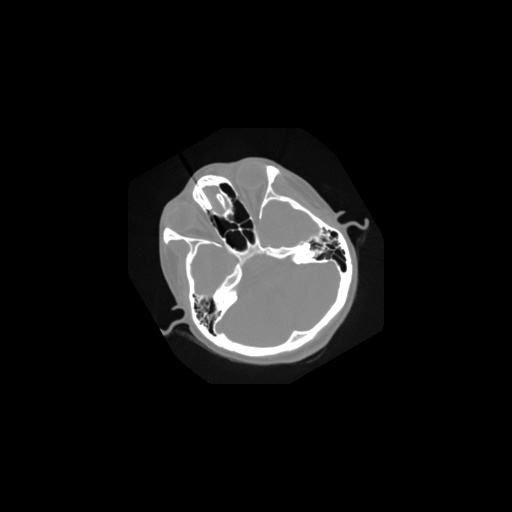
\includegraphics[scale=0.4]{pad-image-2}}
\subfigure[Zero flux Neumann]{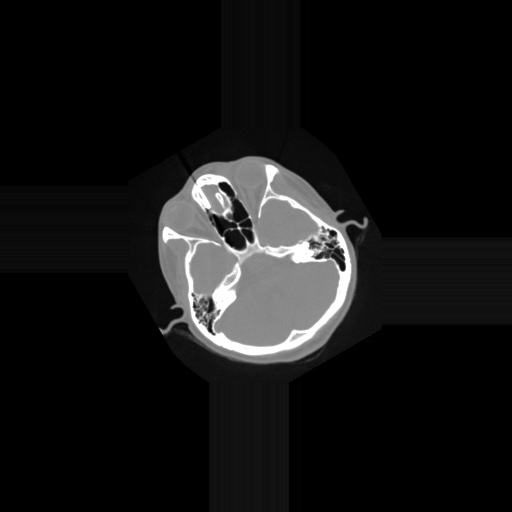
\includegraphics[scale=0.4]{pad-image-zero-flux}}
\subfigure[Mirror]{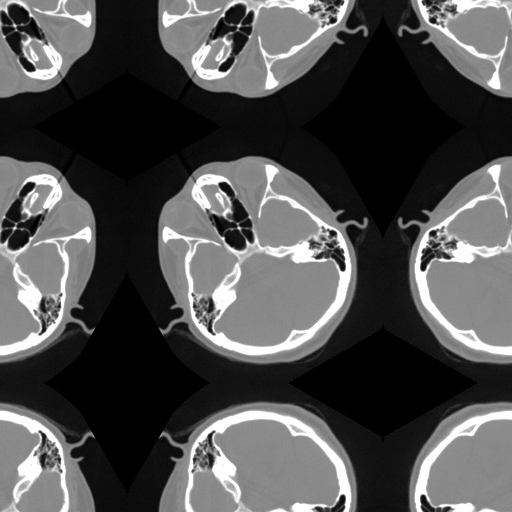
\includegraphics[scale=0.4]{pad-image-mirror}}
\subfigure[Wrap]{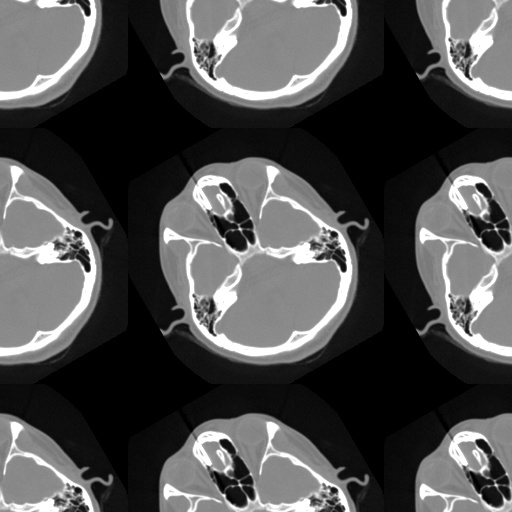
\includegraphics[scale=0.4]{pad-image-wrap}}
\subfigure[Input image]{\includegraphics[scale=0.4]{cthead1}}
\caption{Padding a 256 $\times$ 256 image to a 512 $\times$ 512 one in several ways.\label{fig:padding}}
\end{center}
\end{figure}


\subsection{Normalization}

To preserve the intensity of the pixel in the convolved image, the kernel must be normalized to one
-- the sum of all its pixel is one.

\subsection{Flipping}

The convolution is a flipping transform by nature: the shape of the kernel image can be found in the
convolved image, but flipped on all the axes. To get the same behavior when computing the product
in the frequency domain, the kernel image must be flipped prior to the FFT. See figure \ref{fig:kernel-modifications}.

\begin{figure}[htbp]
\begin{center}
\subfigure[Input image (scaled 20 times)]{
\includegraphics[scale=8]{kernel}}
\subfigure[Zero padded]{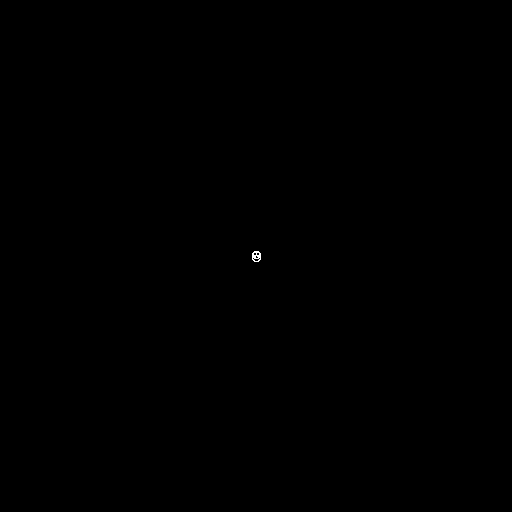
\includegraphics[scale=0.4]{pad-kernel-2}}
\subfigure[Zero padded and flipped]{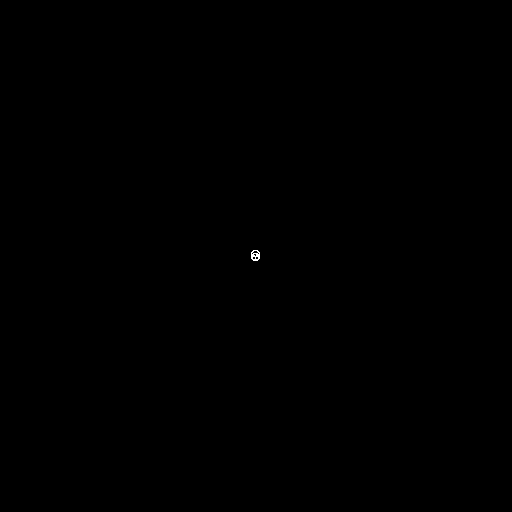
\includegraphics[scale=0.4]{kernel-pad-flip}}
\subfigure[Zero padded, flipped and shifted]{
\includegraphics[scale=0.4]{kernel-pad-flip-shift}}
\caption{Kernel modifications in order to perform the FFT based convolution. Normalization is
only a change in intensity, and thus is not shown here.\label{fig:kernel-modifications}}
\end{center}
\end{figure}

\subsection{Shifting (centering)}

The convolution is usually done with a centered kernel. If the kernel is not centered, the input image
is shifted in the convolved image, by the same shift than the shift of the kernel. However, for the
FFT, the center pixel is the one in the corner, not the one in the center of the image, as is it 
usual for a human. To avoid a shift in the convolved image, the pixels must be shifted to the corner
of the image as expeced by the FFT. See figure \ref{fig:kernel-modifications}.

This shift must be done after the padding, and before the FFT.

Another option, not used here, is to shift the image after the inverse Fourier transform.

\subsection{Fourier transform}

The Fourier transform is performed on the padded input image, and on the normalized, padded, flipped
and shifted kernel.

\subsection{Frequency domain multiplication}

The convolution is performed in the frequency domain, simply by computing the product of the FFT of
the image and of the FFT on the kernel pixel wise.

\subsection{Inverse Fourier transform}

The convolved image in the frequency domain is transformed to the space domain with an inverse Fourier
transform. See figure \ref{fig:image-modifications}.

\begin{figure}[htbp]
\begin{center}
\subfigure[Input image]{\includegraphics[scale=0.4]{cthead1}}
\subfigure[Zero flux Neumann padded]{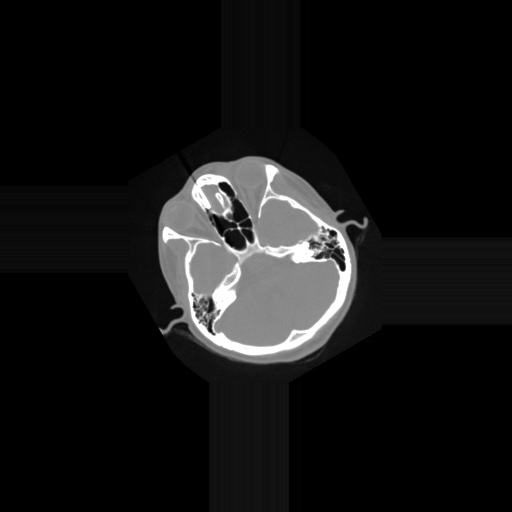
\includegraphics[scale=0.4]{pad-image-zero-flux}}
\subfigure[Convolved, still padded]{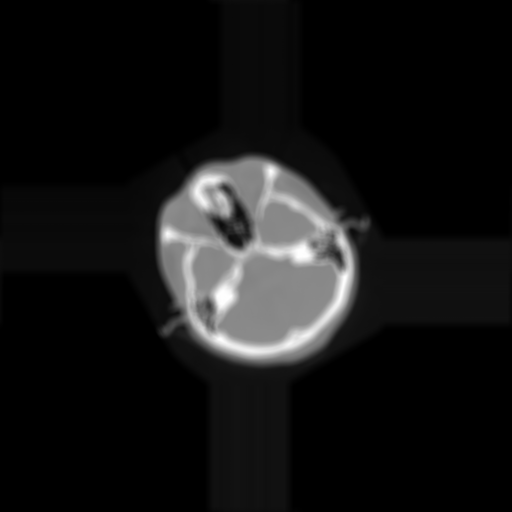
\includegraphics[scale=0.4]{image-pad-convolved}}
\subfigure[Cropped to the input image size]{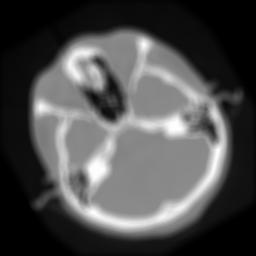
\includegraphics[scale=0.4]{fftconv}}
\caption{The modifications applied to the input image.\label{fig:image-modifications}}
\end{center}
\end{figure}

\subsection{Cropping}

The image is cropped to fit the size of the input image. See figure \ref{fig:image-modifications}.

\section{Implementation}

The step by step transform described in the previous chapter can perfectly be implemented in a pure
ITK pipeline model. The few filters which were missing for this task have been implemented, and some
other have been enhanced to improve their performance.

\subsection{NormalizeToConstantImageFilter}

The normalization to one cannot be done without going outside of the ITK pipeline model at this time.
itk::NormalizeToConstantImageFilter has been added for this task.

This filter is implemented as a minipipeline of two filters:
\begin{itemize}
  \item a itk::StatisticsImageFilter, to compute the sum of the pixels in the image;
  \item a itk::DivideByConstantImageFilter, to actually normalize the pixel values.
\end{itemize}
The use of itk::StatisticsImageFilter only to compute the sum might be {\em a little overkill}. This filter
is only used on the kernel, which is usually quite small, so the performance impact on the whole
FFT based convolution is small.

\subsection{ZeroFluxNeumannPadImageFilter}

The zero flux Neumann padding filter was not implemented in ITK. It has been implemented by modifying
the \verb$ConstantPadImageFilter$ code.

\subsection{FFTPadImageFilter}

The padding step, as described in the previous chapter, has several goals, which lead to a single
image size used to pad both the input image and the kernel.
All the logic is implemented in \verb$itk::FFTPadImageFilter$.

This filter is in charge of padding both images. It requires two input -- the image to convolve and
the kernel. The pad size is computed according to both image sizes.

The image to convolve is simply padded with one of the available method: zeros, zero flux Neumann, mirror
or wrap.

The kernel, however, requires a little more work to be
centered in the padded image, and to make its region match the one of the padded image to convolve.
The padding and the region changes are implemented as a minipipeline of \verb$itk::ConstantPadImageFilter$ and
\verb$itk::ChangeInformationImageFilter$.

\verb$itk::FFTPadImageFilter$ is also able to extend the padded region in order to enhance the FFT
performance, or to make it possible when the FFT possible when it require a size which is a power of
two. FFTW is able to work on any image size, but due to the algorithms useds, produce significantly
more performant result with some specific sizes. The two main reasons are:
\begin{itemize}
  \item the decomposition of images of composite sizes in smaller transforms using the
  Cooley-Tukey algorithm;
  \item the hard coded loop unrolling for the size which are prime numbers up to thirteen.
\end{itemize}
For these reasons, FFTW performs better when the size on each dimension has its greatest prime
factor smaller or equal to thirteen.
The greatest prime factor can be simply computed with the algorithm described in algorithm \ref{greatestPrimeFactor}.

\begin{pseudocode}{isPrime}{n}
\FOREACH x \in [2, \sqrt{n}] \DO 
\BEGIN
  \IF n \% x = 0 \THEN \RETURN \FALSE \\
\END \\
\RETURN \TRUE
\end{pseudocode}

\begin{pseudocode}{greatestPrimeFactor}{n}
\label{greatestPrimeFactor}
x \GETS 2 \\
\WHILE x \leq n \DO
\BEGIN
  \IF n \bmod x = 0 \AND \CALL{isPrime}{x}
  \THEN
    n \GETS n / x
  \ELSE
    v \GETS v + 1
\END \\
\RETURN x
\end{pseudocode}

\verb$FFTPadImageFilter$ can also be used with a single input. This is useful to be able to run a FFT
on an image with a size which is not a power of 2 with the vnl implementation, or to enhance the performance
of the FFTW implementation, without necessairly doing a convolution.

\subsection{FFTW filters enhancements}

ITK provides FFT and inverse FFT filters based on the FFTW library. Those filters had some problems,
or were missing some features. They have been enhanced to fit the needs of the FFT based convolution.

\subsubsection{Thread support}
The FFTW filters were not multithreaded. There are two places where multithreading can take place: the
FFTW execution and the normalization step.

The FFTW execution can be threaded simply by calling \verb$fftwf_plan_with_nthreads(threads);$ or 
\verb$fftwf_plan_with_nthreads(threads);$, depending on the pixel type, before creating the plan. 
\verb$itk::fftw::Proxy$ has been modified to provide this feature: an extra \verb$thread$ parameter,
which defaults
to $1$ to keep the backward compatibility, has been added to the method in charge of creating the plans.
Then the \verb$itk::FFTWComplexConjugateToRealImageFilter$ and
\verb$itk::FFTWRealToComplexConjugateImageFilter$ have
been modified to pass their user defined number of threads to those methods.

In order to implement the threading support in the normalization step in 
\verb$itk::FFTWComplexConjugateToRealImageFilter$, the execution of the FFTW library has been moved to 
\verb$BeforeThreadedGenerateData()$, and the normalization step to \verb$ThreadedGenerateData()$.

\subsubsection{Memory usage reduction}

FFTW filters were using a lot of memory, because they were allocating an internal buffer for the input 
image, and an other one for the output image. Worth, these buffers were not deallocated at the end of
the execution filter, keeping the memory usage very high even when the execution has completed.

I guess the main reasons to do that were:
\begin{itemize}
  \item avoid the destruction of the input. The creation of the FFTW plan, and the execution of FFTW 
  can destroy the input. This is most of the time not acceptable in ITK.
  \item reuse the FFTW plan for a latter run. The plan include the memory location of the input and output
  buffers, so the buffers can't be deallocated, as it may be the case with the filter's input and output images.
\end{itemize}

The destruction of the input can be avoided in the creation plan by using the \verb$FFTW_ESTIMATE$ flag
-- that flag was already used in the implementation. It can also be avoided while running FFTW, for 
the real to complex transform, by also using the flag \verb$FFTW_PRESERVE_INPUT$. So in 
\verb$itk::FFTWRealToComplexConjugateImageFilter$, if the right flags are used, there is no need for
the input buffer.
The case is a bit
more difficult for the complex to real transform: FFTW does not provide any algorithm able to preserve
the input, so the input must be copied to an internal buffer. There is a case however, when we don't
care about destroying the input in ITK: when the \verb$ReleaseDataFlag$ is \verb$ON$ on the input of the filter.
In that case, the input will be deallocated right after the end of the execution of the filter, and so
there is no need to take care of the input -- it can be destroyed by the filter, and then deallocated.
\verb$itk::FFTWRealToComplexConjugateImageFilter$ has been modified to use the input image directly without 
intermediate buffer when \verb$ReleaseDataFlag$ is \verb$ON$. The detection of the \verb$ReleaseDataFlag$
is a bit difficult during the pipeline 
execution: this flag is always modified to \verb$OFF$ before the call to \verb$GenerateData()$ to avoid the 
destruction by a minipipeline. In consequence, the detection of the \verb$ReleaseDataFlag$ is done at an 
earlier stage in the pipeline execution, in \verb$UpdateOutputData()$, and stored in a member variable:
\verb$m_CanUseDestructiveAlgorithm$.

The later reuse of the plan, while sensible when not using the \verb$FFTW_ESTIMATE$ flag, is not much 
interesting when it is used: the time needed to create the plan is very short -- way shorter than the
FFT computation. Also, the number of threads and the image size are stored in the plan, and can't be 
changed later, which doesn't fit well with ITK pipeline model. In the enhanced version, the plan is
not kept between the filters execution, and so no intermediate output buffer are used, decreasing 
significantly the needed memory.

Another reason to create the internal buffer may be the need to align properly the image, to significantly
improve the FFTW performance by using the SIMD operations. The buffer were simply allocated with the
\verb$new$ operator, which is not enough to ensure a proper alignement
on some plateforms, including Microsoft Windows and Linux.


\subsubsection{Code safety}

Only \verb$fftwf_execute(plan);$ and \verb$fftw_execute(plan);$ are thread safe in FFTW -- the other functions
are not thread safe. In consequence, the call to all the other functions has been protected by a 
global lock in the enhanced classes.

Also, the check for the size of the image to know if the plan can be reused may not have been good 
enough, because it was testing only the number of pixels and not the size on all the dimensions. 
The plan is not kept between the execution, so this can not be a problem anymore.

\subsubsection{Still to be done}

There are still some missing features in the FFTW filters. The ones which comes to mind are:
\begin{itemize}
 \item let the user create a plan with \verb$FFTW_PATIENT$, \verb$FFTW_MEASURE$, or
\verb$FFTW_EXHAUSTIVE$, so that FFTW can create better plan with \verb$FFTW_ESTIMATE$ in a
later run;
 \item provide an API to save the FFTW wisdoms.
\end{itemize}


\subsection{RegionFromReferenceImageFilter}

At the end of the convolution, the image is cropped to return to the size of the input image. Again
there is currently no option in ITK to do that fully in the pipeline model. In consequence, a new
filter has been developped for this task.

\verb$itk::RegionFromReferenceImageFilter$ is implemented as a subclass of \verb$itk::ExtractImageFilter$.
This filter requires two inputs -- the first is the image to crop, the second is simply used to get 
the region to extract in the first one. The reference image -- the second input -- is simply expected to
be of type \verb$itk::ImageBase$ with the same dimension than the first one, and so it's type don't
need to be specified in the template parameters.

\subsection{FFTConvolutionImageFilter}

\verb$itk::FFTConvolutionImageFilter$ is a convenient minipipeline filter which groups all the required
filters to make the FFT based convolution in a single and easy to use filter. See figure \ref{fig:conv-pipeline}
for an overview of the minipipeline.
\begin{figure}[htbp]
\centering
\includegraphics[scale=0.5]{conv}
\caption{Internal pipeline of FFTConvolutionImageFilter.\label{fig:conv-pipeline}}
\end{figure}

It sets the \verb$ReleaseDataFlag$ properly to keep the memory usage as low as possible, and propagate the
user specified number of threads.

It also expose the \verb$GreatestPrimeFactor$ accessors from \verb$itk::FFTPadImageFilter$ to let
the user choose between the extra performance added by the padding and the extra memory cost, and
\verb$PadMethod$ from the same filter to let the user choose the padding method -- zero flux Neumann
is used by default.

Finally, the \verb$Normalize$ attribute let the user choose if the kernel must be normalized to one
or not.

\section{Performance}

\subsection{Kernel size}

\subsection{Greatest prime factor}
\label{perf:gpf}
As visible in figure \ref{fig:perf-fftw3}, the FFTW library performs quite differently depending on the
size of the input. A good way to get the best performance seems to be to use the sizes with the greatest
prime factor smaller or equal to 13.

Most of the time, and despite the usual advice to use a size which is a power of two,
those sizes perform significantly better than the closest sizes which are a power of two, probably
because of the smaller impact of the number of pixels in the image.

\begin{figure}[htbp]
\begin{center}
\subfigure[Execution time for an image of size $dim^{3}$.]{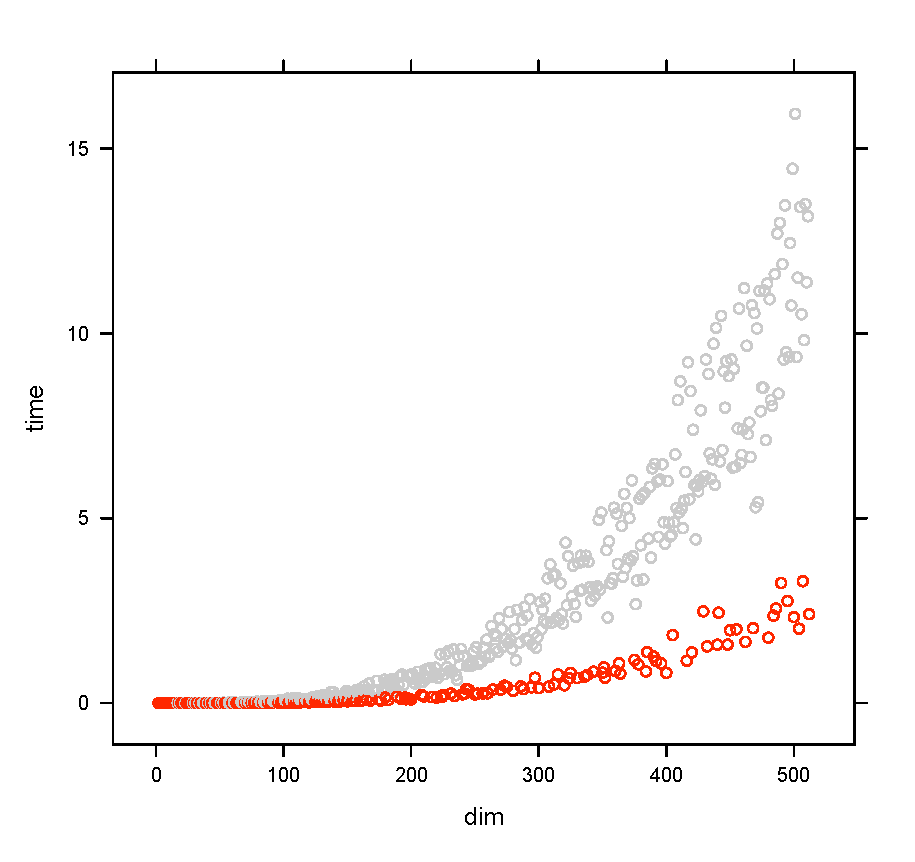
\includegraphics[scale=0.7]{fftw3-time-dim}}
\subfigure[Effect of the image greatest prime factor of the image size (gpf) on the number of pixels
 processed per seconds (ops).]{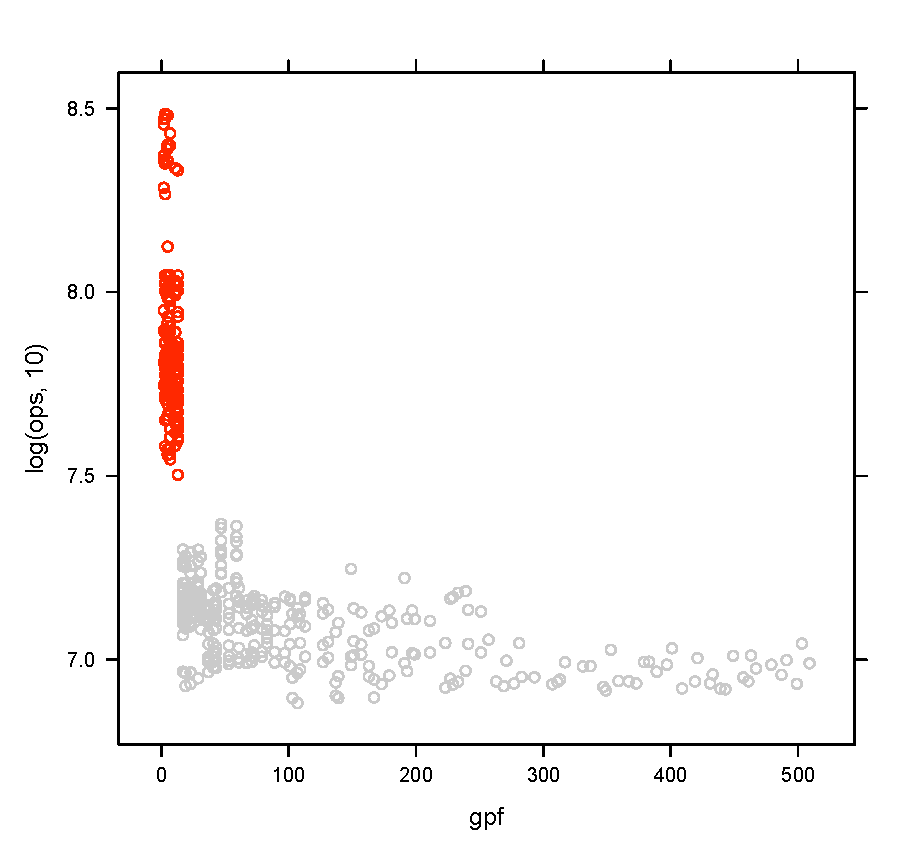
\includegraphics[scale=0.7]{fftw3-ops-gpf}}
\caption{Effect of the image size on the FFTW performance. Red dots are the sizes with a greatest prime
factor smaller or equal to 13. The grey dots are the ones with a greatest prime factor greater than 13.
\label{fig:perf-fftw3}}
\end{center}
\end{figure}

\subsection{Number of threads}

\section{Conclusion}

This contribution provides with an efficient implementation of the convolution transform for large kernels.
The FFTW filters implementations has been significantly enhanced, and a set of reusable tools is provided.

Some other work may be done on this basis -- an non exhaustive list may be:
\begin{itemize}
 \item a binary erosion/dilation based on FFT;
 \item a set of deconvolution filters;
 \item a more memory efficient implementation of the convolution filter using the Overlap-Save algorithm.
\end{itemize}


\appendix



\bibliographystyle{plain}
\bibliography{InsightJournal}
\nocite{ITKSoftwareGuide}

\end{document}

